\documentclass{article}

% Lenguaje y Fuente
\usepackage[spanish]{babel}
\usepackage[utf8x]{inputenc}
\usepackage[T1]{fontenc}
\usepackage[top=1in, bottom=1.25in, left=1.1 in, right=1.1 in]{geometry}
\usepackage{graphicx}
\usepackage{ragged2e}
\usepackage[usenames]{color}
\usepackage{multicol}

% Portada

\title{\textbf{Reporte de la Actividad 10}\\ La Ecuación de Duffing}
\author{Luis Fernando Duarte Gonzalí \\ Universidad de Sonora \\ Física Computacional}
\date{Mayo del 2019}
\begin{document}
\maketitle

% Contenido del Reporte

\section{Introducción}
\subsection{Ecuación de Duffing}
Es una ecuación diferencial no lineal de segundo orden usado como modelo para osciladores forzados y amortiguado. La ecuación está dada por:
\begin{equation}
    \ddot x + \delta \dot x + \alpha x + \beta x^3 = \gamma cos (\omega t)
\end{equation}
donde la función (desconocida) $x = x(t)$ es un desplazamiento en el tiempo $(t)$, $\dot x$ es la primera derivada de $x$ con respecto al tiempo, es decir, la velocidad, y $\ddot x$ es la segunda derivada temporal de $x$, es decir, la aceleración. Los números $\delta$, $alpha$, $\beta$, $\gamma$ y $\omega$ son constantes dadas.

La ecuación describe el movimiento de un oscilador amortiguado con un potencial más complejo que en el movimiento armónico simple (que corresponde al caso de $\beta = \delta = 0$; en términos físicos, modela, por ejemplo, un péndulo de resorte donde la rigidez del resorte no obedece la ley de Hooke.

La ecuación de Duffing es un ejemplo de una sistema dinámico que exhibe un comportamiento caótico. Además, el sistema de Duffing presenta en la respuesta en frecuencia el fenómeno de salto de resonancia que es un tipo de comportamiento de frecuencia de histéresis.

\subsubsection{Parámetros}
$\delta$ controla la cantidad de amortiguamiento, $\alpha$ controla el forzamiento lineal, $\beta$ controla la cantidad de no linearidad en la fuerza restauradora, si $\beta = 0$, la ecuación de Duffin describe un oscilador forzado amortiguado simple. $\gamma$ es la amplitud de la fuerza aplicada como impulso y $\omega$ es la frecuencia angular de la fuerza de impulsora.

En la sigcauiente práctica se busca cia hisreprodutericir la siguiente gráfica que muestra la solución de un sistema muy peculiar con discontinuidad siguiendo rutas distintas incrementando el valor de $\omega$ y disminuyéndolo.

\begin{center}
    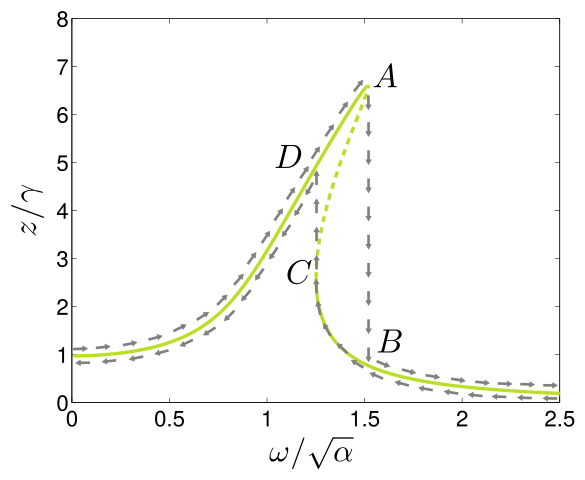
\includegraphics[scale = 0.25]{DuffinG.png}
\end{center}

\section{Resultados}
Usando el método de Runge Kutta de Orden 4 en python se solucionó la ecuación de Duffing, con ayuda de la biblioteca SciPy y la función específica odeint.
Los parámetros para tratar de reproducir la figura 1 fueron los siguientes:
$$\alpha = \gamma = 1.0$$
$$\beta = 0.04$$
$$\delta = 0.1$$
\begin{center}
    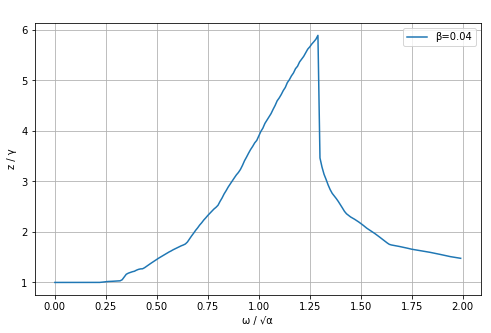
\includegraphics[scale = 0.6]{04.png}
\end{center}
En la cual podemos observar que la amplitud aumenta con la frecuencia, pero después comienza a disminuir también al seguir aumentando.
En las siguientes gráficas se muestra el comportamiento sólo variando la $\beta$ a $-0.003$, $0.01$ y $0.00$.
\begin{center}
    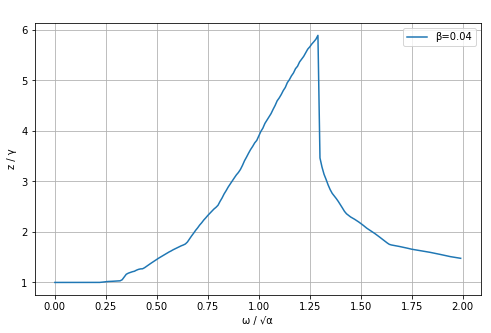
\includegraphics[scale = 0.4]{04.png}
    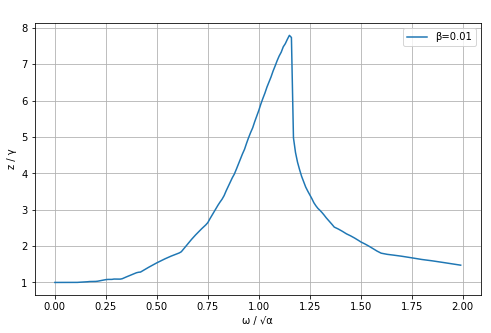
\includegraphics[scale = 0.4]{01.png}
    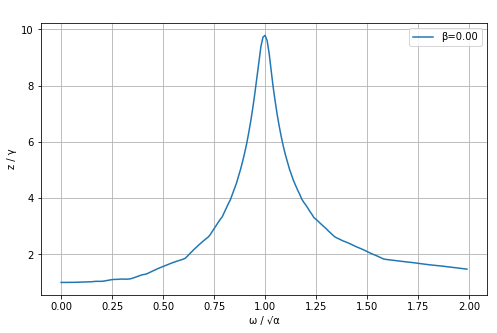
\includegraphics[scale = 0.4]{00.png}
    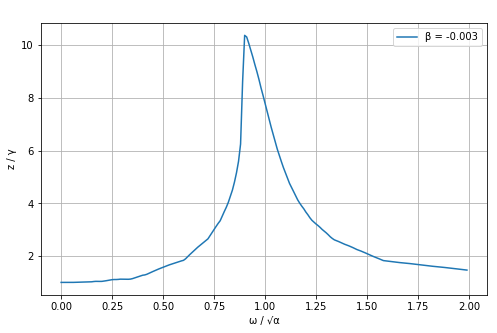
\includegraphics[scale = 0.4]{003.png}
\end{center}

\section{Conclusión}


\section{Referencias}
\begin{itemize}
    \item Duffing Equation. Consultado de Wikipedia. Sitio web:
    
    https://en.wikipedia.org/wiki/Duffing\_equation
    
    \item Función ode de SciPy. Consultado de SciPy.org. Sitio web:
    
    https://docs.scipy.org/doc/scipy/reference/generated/scipy.integrate.ode.html
    
    \item Función odeint de SciPy. Consultado de SciPy.org. Sitio web:
    
    https://docs.scipy.org/doc/scipy/reference/generated/scipy.integrate.odeint.html
    
    \item A modified phase-fitted Runge–Kutta method for the numerical solution of the Schrödinger equation. Consultado de Journal of Mathematical Chemistry. Sitio web:
    
    https://link.springer.com/content/pdf/10.1023/A:1013185619370.pdf
\end{itemize}
\end{document}
